\SourceLeaf{210}auf ihrer Fortsetzung rückwärts, so ist von selbst klar, dass diess keinen Unterschied macht.

Nimmt man dagegen anstatt $A$ einen andern
Anfangspunkt $A'$ auf der Linie $AM\mathinner{.\,.\,.}$,
zieht durch $A'$ zwischen $A'M\mathinner{.\,.\,.}$ und $A'B$
die Gerade $A'P$ in beliebiger Richtung, und
durch einen Punkt $Q$ zwischen $A'$ und $P$
die Gerade $AQ\mathinner{.\,.\,.}$, so wird solche (Definition)
die $BN\mathinner{.\,.\,.}$ schneiden, woraus von selbst klar
ist, dass auch $QP\mathinner{.\,.\,.}$ die $BN\mathinner{.\,.\,.}$ schneiden
wird.

\begin{center}
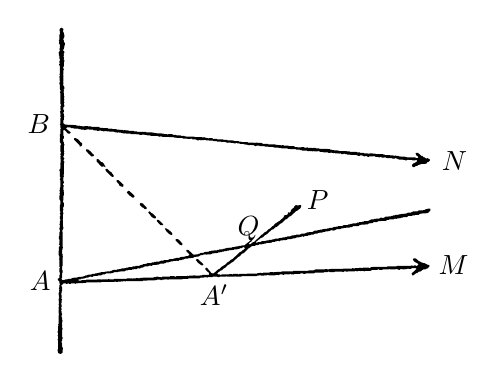
\begin{tikzpicture}[x=0.00567515cm,y=-0.00567515cm]
\fill[even odd rule] (348,497) -- (347,498) -- (347,500) -- (357,510) -- (361,511) -- (362,510) -- (362,507) -- (358,503) -- (358,502) -- (352,497) -- cycle
(323,474) -- (326,479) -- (333,486) -- (338,488) -- (340,486) -- (338,482) -- (331,476) -- (326,473) -- (324,473) -- cycle
(305,455) -- (305,457) -- (313,466) -- (318,466) -- (319,465) -- (319,464) -- (310,455) -- (308,454) -- (306,454) -- cycle
(288,435) -- (286,437) -- (286,438) -- (291,444) -- (291,445) -- (297,450) -- (301,451) -- (303,449) -- (303,447) -- (296,440) -- (293,439) -- (289,435) -- cycle
(269,416) -- (267,418) -- (267,421) -- (272,426) -- (275,427) -- (278,430) -- (281,430) -- (282,429) -- (282,426) -- (275,419) -- (274,417) -- (271,417) -- cycle
(241,389) -- (238,392) -- (238,393) -- (244,400) -- (245,400) -- (250,404) -- (253,404) -- (255,402) -- (254,399) -- (244,390) -- cycle
(216,365) -- (215,366) -- (215,369) -- (220,374) -- (221,377) -- (224,379) -- (229,380) -- (230,379) -- (230,375) -- (219,365) -- cycle
(191,340) -- (190,341) -- (191,345) -- (202,356) -- (203,356) -- (205,358) -- (207,358) -- (208,357) -- (208,354) -- (204,349) -- (204,348) -- (199,345) -- (194,340) -- cycle
(170,319) -- (170,323) -- (181,335) -- (184,335) -- (186,334) -- (190,336) -- (190,334) -- (188,332) -- (187,329) -- (183,325) -- (181,325) -- (174,318) -- (171,318) -- cycle
(148,296) -- (147,297) -- (147,300) -- (150,303) -- (150,304) -- (154,308) -- (155,308) -- (158,312) -- (162,312) -- (164,310) -- (164,308) -- (162,307) -- (156,300) -- (155,300) -- (152,297) -- cycle
(121,271) -- (120,272) -- (120,275) -- (132,287) -- (132,289) -- (133,290) -- (136,289) -- (138,287) -- (138,283) -- (136,281) -- (135,281) -- (129,274) -- (123,271) -- cycle
(88,26) -- (87,30) -- (88,31) -- (88,35) -- (89,37) -- (87,40) -- (87,51) -- (86,52) -- (86,54) -- (87,55) -- (86,59) -- (88,62) -- (88,70) -- (87,71) -- (88,76) -- (85,80) -- (86,82) -- (86,86) -- (87,87) -- (87,93) -- (88,94) -- (88,98) -- (87,99) -- (87,102) -- (88,104) -- (86,106) -- (88,110) -- (88,127) -- (87,128) -- (88,130) -- (88,132) -- (87,133) -- (88,146) -- (87,147) -- (87,150) -- (88,151) -- (88,161) -- (90,166) -- (88,168) -- (89,170) -- (89,194) -- (90,195) -- (90,199) -- (89,200) -- (89,202) -- (90,203) -- (89,205) -- (90,210) -- (88,212) -- (89,214) -- (89,217) -- (90,218) -- (89,220) -- (89,223) -- (90,224) -- (90,226) -- (89,227) -- (89,239) -- (88,240) -- (89,242) -- (89,247) -- (90,248) -- (90,250) -- (89,251) -- (89,262) -- (88,263) -- (88,268) -- (89,269) -- (88,271) -- (88,280) -- (90,283) -- (90,287) -- (89,288) -- (89,301) -- (90,302) -- (90,305) -- (89,306) -- (89,308) -- (90,309) -- (90,311) -- (89,312) -- (89,314) -- (90,315) -- (89,317) -- (90,319) -- (89,332) -- (90,334) -- (89,335) -- (89,340) -- (87,342) -- (87,344) -- (88,345) -- (88,357) -- (89,358) -- (89,361) -- (88,362) -- (88,364) -- (89,365) -- (89,381) -- (88,382) -- (88,387) -- (87,388) -- (88,390) -- (88,394) -- (87,395) -- (88,397) -- (88,399) -- (87,400) -- (87,408) -- (89,411) -- (89,420) -- (88,421) -- (88,434) -- (89,435) -- (89,438) -- (88,439) -- (88,441) -- (89,442) -- (89,445) -- (88,446) -- (88,452) -- (89,453) -- (89,456) -- (88,457) -- (88,463) -- (87,464) -- (88,466) -- (88,471) -- (87,472) -- (87,475) -- (88,476) -- (88,481) -- (87,482) -- (87,490) -- (86,491) -- (86,497) -- (88,499) -- (87,501) -- (87,507) -- (86,509) -- (88,511) -- (88,512) -- (86,515) -- (86,523) -- (85,524) -- (85,532) -- (87,536) -- (87,540) -- (86,542) -- (87,543) -- (87,559) -- (88,560) -- (88,562) -- (87,563) -- (87,571) -- (88,572) -- (88,577) -- (87,578) -- (87,584) -- (83,586) -- (84,589) -- (87,592) -- (87,596) -- (88,597) -- (88,599) -- (87,600) -- (87,605) -- (86,606) -- (86,608) -- (87,609) -- (86,613) -- (87,615) -- (85,618) -- (85,621) -- (86,622) -- (86,625) -- (87,627) -- (86,628) -- (86,631) -- (85,632) -- (85,634) -- (86,635) -- (86,642) -- (85,643) -- (86,645) -- (86,649) -- (85,650) -- (85,654) -- (86,655) -- (85,657) -- (85,663) -- (86,664) -- (86,667) -- (85,668) -- (85,687) -- (84,688) -- (85,691) -- (84,692) -- (84,702) -- (83,703) -- (83,706) -- (84,707) -- (84,712) -- (83,713) -- (84,715) -- (84,720) -- (83,721) -- (83,723) -- (84,724) -- (84,743) -- (83,744) -- (83,748) -- (84,749) -- (84,751) -- (86,753) -- (90,754) -- (94,751) -- (94,744) -- (95,743) -- (95,741) -- (93,738) -- (93,734) -- (92,733) -- (93,731) -- (92,729) -- (92,725) -- (93,724) -- (93,721) -- (94,720) -- (94,717) -- (93,716) -- (93,700) -- (94,699) -- (94,697) -- (93,696) -- (93,688) -- (92,686) -- (93,685) -- (94,679) -- (93,678) -- (93,673) -- (92,672) -- (92,667) -- (93,666) -- (93,664) -- (92,663) -- (92,659) -- (91,658) -- (91,656) -- (92,655) -- (92,653) -- (91,652) -- (91,650) -- (92,649) -- (92,644) -- (91,643) -- (91,641) -- (92,640) -- (92,634) -- (93,633) -- (93,632) -- (91,630) -- (92,628) -- (92,622) -- (91,621) -- (91,619) -- (92,618) -- (92,614) -- (93,613) -- (93,604) -- (91,602) -- (91,601) -- (96,596) -- (101,596) -- (102,597) -- (105,597) -- (106,596) -- (108,596) -- (109,597) -- (112,597) -- (113,596) -- (121,596) -- (123,597) -- (124,596) -- (146,595) -- (147,594) -- (173,594) -- (174,593) -- (176,594) -- (180,594) -- (181,593) -- (210,593) -- (211,592) -- (217,593) -- (218,592) -- (225,592) -- (226,591) -- (228,592) -- (230,591) -- (233,591) -- (234,592) -- (236,591) -- (273,591) -- (274,590) -- (304,589) -- (305,588) -- (313,588) -- (314,589) -- (316,589) -- (317,588) -- (321,588) -- (322,587) -- (328,587) -- (329,588) -- (331,588) -- (332,587) -- (362,587) -- (363,586) -- (375,586) -- (376,585) -- (400,585) -- (403,583) -- (411,583) -- (412,582) -- (419,583) -- (421,581) -- (423,582) -- (429,582) -- (430,581) -- (440,581) -- (441,582) -- (445,582) -- (446,581) -- (459,581) -- (460,580) -- (462,581) -- (479,581) -- (480,580) -- (482,581) -- (494,581) -- (495,580) -- (528,580) -- (529,579) -- (532,579) -- (533,578) -- (544,579) -- (545,578) -- (551,578) -- (552,577) -- (554,577) -- (555,578) -- (570,578) -- (571,577) -- (576,577) -- (578,578) -- (580,576) -- (586,576) -- (587,577) -- (589,577) -- (590,576) -- (593,576) -- (594,575) -- (596,576) -- (602,576) -- (603,575) -- (605,575) -- (606,576) -- (612,576) -- (613,575) -- (625,575) -- (626,574) -- (632,574) -- (633,575) -- (637,575) -- (638,574) -- (656,574) -- (659,572) -- (678,572) -- (679,571) -- (687,571) -- (688,570) -- (691,570) -- (692,571) -- (702,571) -- (703,570) -- (720,570) -- (722,571) -- (724,569) -- (728,569) -- (729,570) -- (732,570) -- (733,569) -- (748,569) -- (749,568) -- (751,568) -- (752,569) -- (754,569) -- (755,568) -- (760,568) -- (761,569) -- (763,568) -- (767,568) -- (768,569) -- (770,569) -- (771,568) -- (783,568) -- (787,566) -- (798,566) -- (799,565) -- (802,565) -- (803,566) -- (809,566) -- (810,565) -- (823,565) -- (824,564) -- (826,564) -- (827,565) -- (838,565) -- (839,564) -- (843,564) -- (844,565) -- (848,566) -- (850,564) -- (859,565) -- (860,564) -- (865,564) -- (866,563) -- (872,564) -- (876,562) -- (884,562) -- (886,564) -- (875,574) -- (876,577) -- (877,578) -- (879,578) -- (884,574) -- (889,572) -- (891,570) -- (894,570) -- (901,565) -- (906,565) -- (908,563) -- (910,563) -- (915,558) -- (915,556) -- (914,555) -- (912,555) -- (904,551) -- (901,551) -- (898,549) -- (896,549) -- (894,547) -- (892,547) -- (885,541) -- (883,540) -- (880,540) -- (878,542) -- (879,545) -- (882,548) -- (888,551) -- (891,554) -- (887,557) -- (885,557) -- (884,556) -- (881,556) -- (880,557) -- (874,556) -- (873,557) -- (842,557) -- (841,558) -- (821,558) -- (820,559) -- (788,559) -- (787,560) -- (784,560) -- (782,562) -- (780,562) -- (779,561) -- (766,561) -- (765,562) -- (759,561) -- (758,562) -- (749,562) -- (748,563) -- (743,562) -- (742,563) -- (691,564) -- (690,565) -- (682,564) -- (681,565) -- (660,565) -- (656,567) -- (645,567) -- (644,568) -- (611,568) -- (610,569) -- (586,569) -- (585,570) -- (567,571) -- (566,572) -- (564,571) -- (558,571) -- (557,572) -- (543,572) -- (542,573) -- (538,573) -- (536,572) -- (535,573) -- (531,573) -- (530,574) -- (490,575) -- (489,576) -- (487,576) -- (486,575) -- (476,575) -- (475,576) -- (468,575) -- (467,576) -- (450,576) -- (449,577) -- (447,577) -- (446,576) -- (442,576) -- (440,574) -- (444,570) -- (445,570) -- (448,567) -- (450,567) -- (454,563) -- (458,561) -- (464,555) -- (468,553) -- (471,550) -- (474,549) -- (487,537) -- (491,535) -- (495,530) -- (500,528) -- (511,517) -- (512,517) -- (517,513) -- (519,513) -- (520,512) -- (524,512) -- (525,511) -- (532,510) -- (535,508) -- (537,509) -- (540,509) -- (541,508) -- (544,508) -- (545,507) -- (548,507) -- (549,506) -- (562,505) -- (564,503) -- (569,503) -- (570,502) -- (573,502) -- (574,501) -- (577,501) -- (579,502) -- (582,500) -- (595,499) -- (598,497) -- (606,497) -- (607,496) -- (615,495) -- (618,493) -- (624,493) -- (625,492) -- (628,492) -- (629,491) -- (632,491) -- (634,492) -- (636,490) -- (642,490) -- (643,489) -- (649,488) -- (650,487) -- (655,487) -- (658,485) -- (663,485) -- (667,483) -- (677,482) -- (678,481) -- (681,481) -- (682,480) -- (687,480) -- (688,479) -- (691,479) -- (695,477) -- (701,478) -- (707,475) -- (715,475) -- (718,473) -- (722,473) -- (723,472) -- (737,471) -- (738,470) -- (742,470) -- (744,468) -- (756,468) -- (758,466) -- (760,466) -- (761,465) -- (777,464) -- (779,462) -- (788,461) -- (790,459) -- (797,459) -- (801,457) -- (806,457) -- (807,456) -- (818,456) -- (820,454) -- (824,454) -- (825,453) -- (834,453) -- (837,451) -- (841,452) -- (842,451) -- (851,450) -- (852,449) -- (855,449) -- (856,448) -- (864,448) -- (868,445) -- (876,445) -- (877,444) -- (882,444) -- (883,443) -- (890,443) -- (892,441) -- (894,441) -- (895,440) -- (910,439) -- (912,438) -- (917,433) -- (917,430) -- (916,429) -- (911,429) -- (910,430) -- (907,430) -- (904,432) -- (901,432) -- (900,433) -- (891,433) -- (888,435) -- (879,435) -- (873,438) -- (867,438) -- (863,440) -- (851,441) -- (850,442) -- (846,442) -- (845,443) -- (839,443) -- (838,444) -- (834,444) -- (833,445) -- (830,445) -- (829,446) -- (824,446) -- (823,447) -- (817,447) -- (812,450) -- (806,449) -- (803,451) -- (796,451) -- (795,452) -- (791,452) -- (790,453) -- (785,453) -- (777,457) -- (769,457) -- (768,458) -- (765,458) -- (764,459) -- (758,459) -- (757,460) -- (754,460) -- (751,462) -- (743,462) -- (742,463) -- (738,463) -- (737,464) -- (734,464) -- (731,466) -- (723,466) -- (719,468) -- (711,468) -- (710,469) -- (701,470) -- (697,472) -- (691,472) -- (690,473) -- (687,473) -- (686,474) -- (680,474) -- (679,475) -- (676,475) -- (675,476) -- (670,476) -- (669,477) -- (665,477) -- (664,478) -- (658,478) -- (654,481) -- (642,482) -- (635,485) -- (629,485) -- (625,487) -- (617,487) -- (616,488) -- (613,488) -- (612,489) -- (607,489) -- (603,491) -- (597,491) -- (596,492) -- (593,492) -- (592,493) -- (587,493) -- (586,494) -- (578,495) -- (577,496) -- (570,496) -- (569,497) -- (563,498) -- (562,499) -- (556,499) -- (555,500) -- (551,500) -- (550,501) -- (539,502) -- (536,504) -- (531,504) -- (530,505) -- (527,505) -- (526,504) -- (533,498) -- (534,498) -- (537,495) -- (542,493) -- (547,488) -- (550,487) -- (562,476) -- (566,475) -- (571,470) -- (573,470) -- (582,462) -- (585,461) -- (593,453) -- (596,452) -- (601,447) -- (605,445) -- (617,434) -- (620,433) -- (623,430) -- (624,430) -- (626,428) -- (628,424) -- (628,422) -- (627,421) -- (623,421) -- (622,422) -- (616,421) -- (612,425) -- (612,426) -- (605,432) -- (605,435) -- (602,438) -- (599,437) -- (598,438) -- (598,441) -- (596,443) -- (590,444) -- (589,445) -- (589,448) -- (585,452) -- (584,452) -- (580,456) -- (569,463) -- (565,468) -- (564,468) -- (559,473) -- (555,475) -- (550,480) -- (546,482) -- (541,487) -- (540,487) -- (522,504) -- (520,504) -- (514,509) -- (513,509) -- (511,507) -- (511,506) -- (518,501) -- (518,500) -- (516,499) -- (501,511) -- (495,511) -- (494,512) -- (489,512) -- (488,513) -- (480,514) -- (479,515) -- (474,515) -- (473,516) -- (461,517) -- (460,518) -- (457,518) -- (456,519) -- (453,519) -- (452,520) -- (445,520) -- (444,521) -- (441,521) -- (440,522) -- (427,523) -- (426,524) -- (423,524) -- (422,525) -- (412,526) -- (409,528) -- (403,528) -- (400,530) -- (398,530) -- (397,531) -- (392,531) -- (391,532) -- (387,532) -- (375,521) -- (372,521) -- (371,522) -- (371,524) -- (378,531) -- (378,532) -- (375,535) -- (370,535) -- (369,536) -- (366,536) -- (365,537) -- (359,537) -- (355,539) -- (348,539) -- (347,540) -- (344,540) -- (341,542) -- (333,542) -- (330,544) -- (321,544) -- (320,545) -- (315,545) -- (312,547) -- (300,548) -- (299,549) -- (295,549) -- (291,551) -- (284,551) -- (283,552) -- (280,552) -- (279,553) -- (275,553) -- (272,555) -- (269,555) -- (265,557) -- (258,557) -- (257,558) -- (252,558) -- (248,560) -- (242,560) -- (241,561) -- (237,561) -- (236,562) -- (225,563) -- (224,564) -- (216,565) -- (215,566) -- (208,566) -- (201,569) -- (194,569) -- (193,570) -- (189,570) -- (188,571) -- (180,571) -- (179,572) -- (175,572) -- (174,573) -- (171,573) -- (170,574) -- (167,574) -- (166,575) -- (161,575) -- (160,576) -- (150,577) -- (149,578) -- (147,578) -- (140,581) -- (128,582) -- (127,583) -- (120,583) -- (119,584) -- (116,584) -- (113,586) -- (106,586) -- (105,587) -- (101,587) -- (100,588) -- (94,589) -- (92,587) -- (92,584) -- (93,583) -- (93,573) -- (94,572) -- (94,567) -- (93,566) -- (93,558) -- (94,557) -- (94,538) -- (95,537) -- (94,535) -- (94,531) -- (93,530) -- (93,521) -- (94,520) -- (94,517) -- (95,516) -- (94,514) -- (94,481) -- (93,479) -- (96,473) -- (96,470) -- (95,469) -- (95,455) -- (94,453) -- (95,452) -- (95,442) -- (96,441) -- (96,438) -- (95,437) -- (95,433) -- (96,432) -- (96,430) -- (95,429) -- (95,427) -- (97,423) -- (97,417) -- (95,413) -- (95,411) -- (96,410) -- (96,400) -- (97,399) -- (97,392) -- (96,391) -- (97,389) -- (96,387) -- (96,380) -- (97,378) -- (95,376) -- (95,374) -- (97,371) -- (97,369) -- (96,368) -- (96,365) -- (95,363) -- (96,362) -- (96,358) -- (97,357) -- (96,353) -- (97,352) -- (97,327) -- (98,326) -- (98,324) -- (96,322) -- (97,318) -- (98,317) -- (98,316) -- (96,314) -- (96,311) -- (97,310) -- (97,307) -- (98,306) -- (97,304) -- (97,302) -- (98,301) -- (97,299) -- (97,288) -- (98,287) -- (98,285) -- (97,284) -- (97,281) -- (96,280) -- (96,277) -- (95,276) -- (95,274) -- (97,271) -- (97,267) -- (96,266) -- (96,257) -- (95,255) -- (97,253) -- (99,253) -- (106,261) -- (110,261) -- (112,259) -- (112,258) -- (102,250) -- (102,249) -- (104,247) -- (111,247) -- (114,249) -- (119,249) -- (120,250) -- (129,250) -- (130,251) -- (134,251) -- (135,252) -- (142,252) -- (143,253) -- (152,251) -- (153,252) -- (162,252) -- (164,254) -- (171,254) -- (172,255) -- (180,254) -- (181,255) -- (184,255) -- (185,256) -- (192,255) -- (193,256) -- (211,257) -- (212,258) -- (215,258) -- (216,259) -- (220,258) -- (221,259) -- (225,259) -- (226,260) -- (230,260) -- (231,261) -- (235,260) -- (236,261) -- (246,261) -- (247,262) -- (259,262) -- (260,263) -- (266,263) -- (267,264) -- (277,263) -- (278,264) -- (282,264) -- (283,265) -- (290,265) -- (291,266) -- (307,266) -- (310,268) -- (315,267) -- (316,268) -- (343,269) -- (344,270) -- (363,271) -- (364,272) -- (373,272) -- (374,273) -- (380,273) -- (381,272) -- (383,272) -- (385,274) -- (392,274) -- (396,276) -- (399,276) -- (400,275) -- (402,275) -- (403,276) -- (414,275) -- (415,276) -- (431,277) -- (432,278) -- (439,278) -- (440,279) -- (449,279) -- (450,280) -- (456,279) -- (457,280) -- (460,280) -- (462,282) -- (464,281) -- (470,281) -- (471,282) -- (476,282) -- (477,283) -- (481,283) -- (482,282) -- (484,282) -- (485,283) -- (490,283) -- (491,284) -- (499,284) -- (500,285) -- (508,286) -- (509,287) -- (513,287) -- (514,286) -- (516,286) -- (517,287) -- (522,287) -- (525,289) -- (527,289) -- (528,288) -- (534,288) -- (535,289) -- (546,289) -- (547,290) -- (565,291) -- (566,292) -- (583,293) -- (584,294) -- (597,294) -- (598,295) -- (602,295) -- (603,296) -- (616,296) -- (617,297) -- (625,297) -- (626,298) -- (629,298) -- (630,299) -- (641,299) -- (642,300) -- (652,300) -- (653,301) -- (655,300) -- (657,300) -- (658,301) -- (664,301) -- (665,300) -- (667,300) -- (671,302) -- (677,302) -- (678,303) -- (688,303) -- (689,304) -- (693,304) -- (695,303) -- (696,304) -- (699,304) -- (700,305) -- (702,304) -- (704,305) -- (711,305) -- (712,306) -- (716,305) -- (718,307) -- (722,307) -- (723,306) -- (725,306) -- (726,307) -- (730,307) -- (731,308) -- (753,309) -- (755,311) -- (758,311) -- (759,310) -- (765,310) -- (769,312) -- (774,311) -- (777,313) -- (779,313) -- (780,312) -- (789,312) -- (791,311) -- (795,313) -- (800,313) -- (801,314) -- (804,314) -- (806,313) -- (809,315) -- (813,315) -- (814,314) -- (816,314) -- (820,316) -- (831,316) -- (832,317) -- (837,317) -- (838,316) -- (840,316) -- (847,319) -- (856,319) -- (857,320) -- (860,320) -- (861,321) -- (863,321) -- (867,319) -- (869,320) -- (876,320) -- (877,321) -- (883,321) -- (884,320) -- (886,320) -- (887,321) -- (887,323) -- (885,325) -- (879,328) -- (876,331) -- (876,334) -- (879,336) -- (881,336) -- (885,333) -- (888,333) -- (890,331) -- (892,331) -- (893,330) -- (896,330) -- (897,329) -- (905,329) -- (906,328) -- (908,328) -- (911,324) -- (913,324) -- (916,321) -- (916,319) -- (911,316) -- (907,317) -- (904,314) -- (902,314) -- (899,311) -- (897,311) -- (889,304) -- (885,304) -- (884,305) -- (885,309) -- (890,313) -- (890,314) -- (888,316) -- (886,316) -- (882,314) -- (864,314) -- (863,313) -- (846,312) -- (845,311) -- (840,311) -- (839,310) -- (835,311) -- (834,310) -- (827,310) -- (826,309) -- (816,309) -- (815,308) -- (812,308) -- (811,307) -- (795,307) -- (794,306) -- (788,306) -- (787,305) -- (777,306) -- (776,305) -- (768,305) -- (767,304) -- (760,304) -- (759,303) -- (753,303) -- (752,302) -- (737,302) -- (736,301) -- (730,301) -- (729,300) -- (713,300) -- (712,299) -- (697,298) -- (696,297) -- (693,297) -- (692,296) -- (687,296) -- (686,295) -- (669,295) -- (668,294) -- (661,294) -- (660,293) -- (655,293) -- (653,294) -- (652,293) -- (643,293) -- (642,292) -- (636,293) -- (634,291) -- (629,291) -- (628,292) -- (620,292) -- (619,291) -- (614,291) -- (612,289) -- (600,289) -- (599,288) -- (589,288) -- (588,287) -- (585,287) -- (583,288) -- (582,287) -- (577,287) -- (576,286) -- (571,286) -- (570,285) -- (554,285) -- (553,284) -- (543,284) -- (539,282) -- (531,282) -- (530,281) -- (522,282) -- (521,281) -- (509,281) -- (508,280) -- (495,280) -- (494,279) -- (489,279) -- (488,278) -- (479,278) -- (478,277) -- (475,277) -- (474,276) -- (463,276) -- (462,275) -- (454,275) -- (453,274) -- (440,274) -- (439,273) -- (431,273) -- (429,271) -- (422,271) -- (420,272) -- (419,271) -- (416,271) -- (415,270) -- (412,270) -- (411,269) -- (407,270) -- (406,269) -- (390,269) -- (389,268) -- (371,268) -- (370,267) -- (367,267) -- (366,266) -- (359,266) -- (358,265) -- (349,265) -- (348,264) -- (342,264) -- (338,262) -- (331,262) -- (330,263) -- (328,263) -- (327,262) -- (321,262) -- (320,261) -- (300,260) -- (299,259) -- (295,259) -- (294,258) -- (281,258) -- (280,257) -- (261,257) -- (260,256) -- (254,256) -- (253,255) -- (242,255) -- (241,254) -- (235,254) -- (234,253) -- (230,254) -- (229,253) -- (215,252) -- (214,251) -- (206,251) -- (205,250) -- (202,250) -- (200,251) -- (199,250) -- (196,250) -- (195,249) -- (185,249) -- (184,248) -- (178,248) -- (174,246) -- (159,246) -- (158,245) -- (151,245) -- (150,244) -- (138,245) -- (137,244) -- (133,244) -- (132,243) -- (129,244) -- (128,243) -- (125,243) -- (124,242) -- (100,241) -- (96,238) -- (96,231) -- (97,230) -- (97,224) -- (98,223) -- (97,221) -- (97,217) -- (96,216) -- (96,213) -- (97,212) -- (97,209) -- (96,208) -- (96,202) -- (98,200) -- (98,197) -- (97,196) -- (97,193) -- (98,192) -- (98,190) -- (97,189) -- (97,187) -- (98,186) -- (97,181) -- (98,180) -- (98,178) -- (97,177) -- (97,170) -- (96,169) -- (97,165) -- (96,163) -- (98,161) -- (98,157) -- (95,152) -- (96,150) -- (96,145) -- (95,144) -- (96,142) -- (96,130) -- (95,128) -- (96,127) -- (96,119) -- (97,118) -- (95,112) -- (97,110) -- (97,101) -- (98,100) -- (98,97) -- (96,95) -- (97,93) -- (97,91) -- (96,90) -- (97,85) -- (96,83) -- (98,80) -- (98,78) -- (95,75) -- (95,74) -- (97,71) -- (97,69) -- (98,68) -- (98,64) -- (99,63) -- (99,58) -- (97,56) -- (97,53) -- (96,52) -- (96,49) -- (98,45) -- (98,40) -- (97,39) -- (97,36) -- (95,33) -- (96,27) -- (92,24) -- cycle
(502,517) -- (502,518) -- (499,521) -- (498,521) -- (494,525) -- (491,526) -- (474,542) -- (471,543) -- (467,547) -- (464,548) -- (458,554) -- (450,559) -- (445,564) -- (442,565) -- (433,573) -- (431,574) -- (427,573) -- (417,561) -- (414,562) -- (413,564) -- (416,567) -- (416,568) -- (421,572) -- (422,574) -- (422,576) -- (421,577) -- (407,577) -- (406,578) -- (402,578) -- (401,579) -- (391,579) -- (390,578) -- (387,578) -- (386,579) -- (377,579) -- (376,580) -- (373,579) -- (372,580) -- (349,580) -- (348,581) -- (345,581) -- (344,580) -- (335,580) -- (334,581) -- (317,581) -- (315,583) -- (313,582) -- (309,582) -- (308,581) -- (304,581) -- (303,582) -- (299,582) -- (298,583) -- (274,583) -- (273,584) -- (267,584) -- (266,585) -- (259,584) -- (258,585) -- (252,585) -- (251,586) -- (249,585) -- (238,585) -- (237,586) -- (210,586) -- (209,587) -- (199,587) -- (197,586) -- (196,587) -- (182,587) -- (181,588) -- (179,587) -- (172,587) -- (171,588) -- (147,588) -- (146,589) -- (137,589) -- (136,590) -- (130,590) -- (129,589) -- (130,587) -- (134,587) -- (137,585) -- (140,586) -- (141,585) -- (143,585) -- (147,583) -- (151,583) -- (155,581) -- (158,581) -- (160,582) -- (163,580) -- (173,579) -- (174,578) -- (180,578) -- (184,576) -- (188,576) -- (191,574) -- (202,574) -- (203,573) -- (206,573) -- (210,571) -- (218,571) -- (219,570) -- (223,570) -- (224,569) -- (233,569) -- (236,567) -- (240,567) -- (241,566) -- (249,566) -- (250,565) -- (253,565) -- (254,564) -- (260,564) -- (262,562) -- (267,563) -- (270,561) -- (273,561) -- (278,558) -- (285,558) -- (289,556) -- (293,557) -- (296,555) -- (304,555) -- (305,554) -- (309,554) -- (313,552) -- (321,552) -- (322,551) -- (324,551) -- (326,549) -- (331,549) -- (332,548) -- (335,548) -- (336,547) -- (341,547) -- (342,546) -- (348,546) -- (349,545) -- (353,546) -- (355,544) -- (360,544) -- (361,543) -- (364,543) -- (368,541) -- (374,541) -- (375,540) -- (386,539) -- (389,537) -- (398,536) -- (403,533) -- (407,533) -- (408,532) -- (411,532) -- (412,531) -- (414,531) -- (415,532) -- (417,532) -- (418,531) -- (426,531) -- (430,529) -- (441,528) -- (442,527) -- (450,526) -- (451,525) -- (455,525) -- (456,524) -- (461,524) -- (462,523) -- (466,523) -- (467,522) -- (473,522) -- (474,521) -- (477,521) -- (478,520) -- (485,520) -- (486,519) -- (489,519) -- (492,517) -- (495,517) -- (498,515) -- (500,515) -- cycle
(393,543) -- (393,545) -- (395,547) -- (395,548) -- (402,554) -- (403,554) -- (405,556) -- (407,556) -- (409,554) -- (409,553) -- (397,542) -- (394,542) -- cycle;
\node[inner sep=0pt] at (41,239) {$B$};
\node[inner sep=0pt] at (971,323) {$N$};
\node[inner sep=0pt] at (665,409) {$P$};
\node[inner sep=0pt] at (510,473) {$Q$};
\node[inner sep=0pt] at (44,591) {$A$};
\node[inner sep=0pt] at (433,622) {$A'$};
\node[inner sep=0pt] at (969,555) {$M$};
\end{tikzpicture}

\end{center}

Nimmt man aber $A'$ auf der rückwärts fortgesetzten $AM\mathinner{.\,.\,.}$ und zieht

\begin{center}
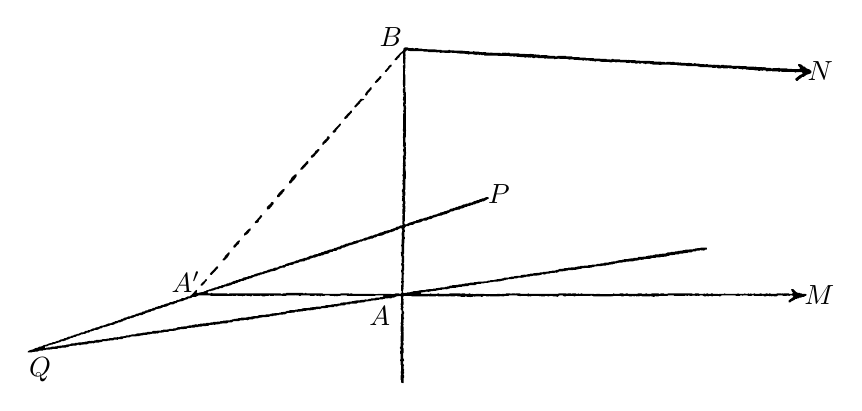
\begin{tikzpicture}[x=0.00543197cm,y=-0.00543197cm]
\fill[even odd rule] (439,601) -- (437,601) -- (435,603) -- (435,604) -- (427,611) -- (427,612) -- (425,614) -- (426,616) -- (429,616) -- (436,609) -- (436,608) -- (440,604) -- (440,602) -- cycle
(465,571) -- (463,571) -- (447,588) -- (447,589) -- (449,591) -- (451,591) -- (466,575) -- (466,572) -- cycle
(492,538) -- (491,538) -- (482,547) -- (481,550) -- (477,554) -- (477,556) -- (478,557) -- (481,557) -- (489,549) -- (493,542) -- (493,539) -- cycle
(516,510) -- (512,512) -- (502,523) -- (502,526) -- (503,527) -- (506,527) -- (509,524) -- (509,523) -- (515,518) -- (516,514) -- (517,513) -- (517,511) -- cycle
(541,482) -- (536,485) -- (532,489) -- (532,490) -- (528,493) -- (527,495) -- (527,498) -- (528,499) -- (534,496) -- (539,491) -- (539,490) -- (542,487) -- (542,483) -- cycle
(567,451) -- (566,451) -- (563,454) -- (563,455) -- (558,460) -- (558,461) -- (552,467) -- (552,469) -- (553,470) -- (558,469) -- (561,467) -- (562,463) -- (569,455) -- (569,453) -- cycle
(595,421) -- (592,420) -- (589,423) -- (589,424) -- (580,432) -- (580,436) -- (582,438) -- (586,437) -- (593,429) -- (593,428) -- (596,425) -- (596,422) -- cycle
(621,390) -- (617,391) -- (607,401) -- (607,402) -- (604,405) -- (604,408) -- (605,409) -- (608,409) -- (610,408) -- (611,406) -- (617,400) -- (617,399) -- (621,395) -- (621,393) -- (622,392) -- cycle
(649,356) -- (646,356) -- (638,363) -- (635,369) -- (632,372) -- (632,376) -- (633,377) -- (636,377) -- (647,365) -- (650,360) -- (650,357) -- cycle
(676,325) -- (674,325) -- (660,340) -- (660,341) -- (658,343) -- (659,345) -- (662,345) -- (664,344) -- (677,330) -- (677,326) -- cycle
(702,297) -- (699,297) -- (696,300) -- (695,300) -- (693,302) -- (691,306) -- (683,313) -- (683,316) -- (684,317) -- (687,317) -- (693,312) -- (693,311) -- (703,300) -- (703,298) -- cycle
(725,267) -- (722,267) -- (721,268) -- (720,272) -- (718,274) -- (717,274) -- (710,282) -- (710,286) -- (711,287) -- (712,287) -- (717,282) -- (718,282) -- (727,272) -- (727,269) -- cycle
(752,237) -- (751,237) -- (734,255) -- (734,257) -- (735,258) -- (739,258) -- (743,254) -- (743,252) -- (752,242) -- (753,240) -- (753,238) -- cycle
(778,207) -- (776,207) -- (774,209) -- (774,210) -- (772,212) -- (771,212) -- (762,222) -- (761,224) -- (762,226) -- (765,226) -- (770,222) -- (770,221) -- (779,211) -- (779,208) -- cycle
(808,180) -- (800,179) -- (785,196) -- (785,198) -- (786,199) -- (788,199) -- (796,191) -- (798,190) -- (798,188) -- (803,183) -- (807,182) -- cycle
(824,152) -- (823,152) -- (812,164) -- (810,168) -- (810,170) -- (812,172) -- (813,172) -- (816,169) -- (816,167) -- (825,157) -- (825,153) -- cycle
(847,126) -- (845,126) -- (833,139) -- (833,141) -- (834,142) -- (836,142) -- (838,140) -- (839,140) -- (848,130) -- (848,127) -- cycle
(871,99) -- (867,101) -- (864,104) -- (864,105) -- (856,114) -- (857,116) -- (860,116) -- (867,108) -- (867,107) -- (872,103) -- (872,100) -- cycle
(1853,114) -- (1848,110) -- (1845,110) -- (1843,108) -- (1841,108) -- (1838,104) -- (1835,104) -- (1830,99) -- (1828,99) -- (1827,98) -- (1823,98) -- (1822,99) -- (1822,101) -- (1827,107) -- (1827,108) -- (1825,110) -- (1808,110) -- (1807,109) -- (1797,109) -- (1796,108) -- (1780,108) -- (1779,107) -- (1759,108) -- (1758,107) -- (1748,107) -- (1747,106) -- (1744,106) -- (1743,105) -- (1739,106) -- (1738,105) -- (1725,105) -- (1724,104) -- (1722,104) -- (1721,105) -- (1719,104) -- (1702,104) -- (1701,103) -- (1687,103) -- (1686,102) -- (1667,102) -- (1666,101) -- (1655,101) -- (1654,100) -- (1652,101) -- (1650,101) -- (1649,100) -- (1643,100) -- (1642,101) -- (1639,101) -- (1638,100) -- (1627,100) -- (1626,99) -- (1624,100) -- (1620,100) -- (1619,99) -- (1611,99) -- (1610,98) -- (1603,99) -- (1602,98) -- (1592,98) -- (1591,97) -- (1583,97) -- (1582,96) -- (1580,96) -- (1579,97) -- (1574,97) -- (1573,96) -- (1569,96) -- (1568,95) -- (1565,95) -- (1564,96) -- (1559,96) -- (1558,95) -- (1549,95) -- (1548,94) -- (1544,95) -- (1543,94) -- (1534,94) -- (1533,93) -- (1528,93) -- (1527,94) -- (1525,93) -- (1515,93) -- (1514,94) -- (1511,94) -- (1510,93) -- (1502,93) -- (1501,92) -- (1495,92) -- (1493,93) -- (1492,92) -- (1485,92) -- (1484,91) -- (1443,90) -- (1442,89) -- (1428,89) -- (1427,88) -- (1423,89) -- (1422,88) -- (1406,88) -- (1405,87) -- (1391,87) -- (1390,86) -- (1387,86) -- (1385,88) -- (1384,88) -- (1383,87) -- (1375,87) -- (1374,86) -- (1360,86) -- (1359,85) -- (1345,85) -- (1344,84) -- (1326,84) -- (1325,83) -- (1312,83) -- (1311,82) -- (1296,82) -- (1293,80) -- (1280,80) -- (1279,79) -- (1260,79) -- (1259,80) -- (1254,80) -- (1253,79) -- (1241,79) -- (1240,78) -- (1236,78) -- (1235,77) -- (1222,77) -- (1220,78) -- (1217,76) -- (1209,76) -- (1208,75) -- (1205,76) -- (1204,75) -- (1199,75) -- (1198,74) -- (1195,74) -- (1194,75) -- (1188,75) -- (1186,74) -- (1184,75) -- (1183,74) -- (1171,74) -- (1170,73) -- (1149,73) -- (1146,71) -- (1144,72) -- (1139,72) -- (1138,71) -- (1134,72) -- (1132,71) -- (1129,73) -- (1127,73) -- (1126,72) -- (1108,72) -- (1107,71) -- (1103,71) -- (1101,72) -- (1100,71) -- (1093,71) -- (1092,70) -- (1086,70) -- (1084,71) -- (1083,70) -- (1077,70) -- (1076,69) -- (1066,69) -- (1065,68) -- (1063,68) -- (1062,69) -- (1054,69) -- (1053,68) -- (1044,68) -- (1043,67) -- (1009,66) -- (1008,65) -- (1005,65) -- (1004,66) -- (989,66) -- (988,65) -- (978,65) -- (977,64) -- (944,63) -- (943,62) -- (935,62) -- (934,61) -- (927,61) -- (925,62) -- (921,60) -- (919,61) -- (914,61) -- (913,60) -- (910,60) -- (909,59) -- (903,59) -- (900,61) -- (899,66) -- (894,71) -- (893,71) -- (879,86) -- (879,88) -- (880,89) -- (883,89) -- (886,86) -- (886,85) -- (890,82) -- (891,79) -- (896,73) -- (898,73) -- (899,74) -- (899,96) -- (900,97) -- (900,100) -- (898,102) -- (898,105) -- (899,106) -- (899,122) -- (898,123) -- (899,125) -- (899,135) -- (898,136) -- (898,146) -- (899,147) -- (899,151) -- (900,152) -- (900,154) -- (898,157) -- (898,163) -- (900,167) -- (899,169) -- (900,171) -- (900,174) -- (899,175) -- (899,179) -- (898,181) -- (900,184) -- (900,187) -- (899,188) -- (899,196) -- (900,197) -- (900,206) -- (899,207) -- (899,209) -- (900,210) -- (900,213) -- (899,214) -- (899,249) -- (898,250) -- (898,254) -- (900,258) -- (899,259) -- (899,267) -- (898,268) -- (898,270) -- (899,271) -- (899,287) -- (898,289) -- (900,292) -- (900,296) -- (899,297) -- (899,302) -- (900,303) -- (900,311) -- (898,313) -- (898,316) -- (899,317) -- (899,329) -- (898,330) -- (898,332) -- (899,333) -- (898,335) -- (899,341) -- (898,342) -- (898,352) -- (899,354) -- (897,357) -- (897,359) -- (898,360) -- (898,369) -- (897,370) -- (897,372) -- (898,373) -- (898,375) -- (897,376) -- (897,379) -- (898,380) -- (898,389) -- (896,393) -- (896,396) -- (897,397) -- (897,403) -- (898,404) -- (898,405) -- (896,407) -- (897,409) -- (896,417) -- (898,419) -- (898,425) -- (897,426) -- (897,428) -- (898,429) -- (897,431) -- (898,433) -- (898,436) -- (897,437) -- (897,448) -- (898,449) -- (898,451) -- (897,452) -- (897,463) -- (898,464) -- (897,466) -- (897,471) -- (898,473) -- (896,475) -- (893,475) -- (888,478) -- (884,478) -- (882,480) -- (878,482) -- (876,482) -- (873,484) -- (871,484) -- (868,486) -- (865,486) -- (864,487) -- (861,487) -- (860,488) -- (856,488) -- (851,491) -- (845,492) -- (837,496) -- (834,496) -- (828,499) -- (824,499) -- (821,501) -- (819,501) -- (816,503) -- (810,504) -- (802,508) -- (799,508) -- (795,510) -- (791,510) -- (787,512) -- (784,512) -- (779,515) -- (772,516) -- (769,518) -- (765,518) -- (762,520) -- (760,520) -- (758,522) -- (754,522) -- (750,525) -- (748,525) -- (741,528) -- (738,528) -- (736,530) -- (734,530) -- (733,531) -- (729,531) -- (728,532) -- (726,532) -- (719,535) -- (716,535) -- (713,537) -- (708,538) -- (705,540) -- (702,540) -- (699,542) -- (692,543) -- (686,546) -- (682,546) -- (672,551) -- (668,551) -- (667,552) -- (656,555) -- (653,557) -- (649,557) -- (646,559) -- (625,565) -- (621,568) -- (619,568) -- (615,570) -- (611,570) -- (604,574) -- (599,574) -- (593,577) -- (589,577) -- (588,578) -- (583,579) -- (580,581) -- (572,583) -- (569,585) -- (564,585) -- (563,586) -- (552,589) -- (549,591) -- (544,592) -- (541,594) -- (537,594) -- (533,596) -- (526,597) -- (524,599) -- (522,599) -- (520,601) -- (516,601) -- (512,603) -- (509,603) -- (506,605) -- (503,605) -- (496,609) -- (493,609) -- (491,611) -- (487,611) -- (485,613) -- (482,613) -- (478,615) -- (475,615) -- (472,617) -- (469,617) -- (463,620) -- (459,620) -- (456,622) -- (451,623) -- (448,625) -- (445,625) -- (444,626) -- (439,627) -- (437,629) -- (435,629) -- (431,631) -- (423,632) -- (422,633) -- (417,633) -- (416,632) -- (417,627) -- (415,626) -- (409,632) -- (409,633) -- (400,641) -- (396,641) -- (388,645) -- (382,645) -- (378,648) -- (376,648) -- (375,649) -- (371,649) -- (367,652) -- (364,652) -- (360,654) -- (353,655) -- (351,657) -- (345,658) -- (338,661) -- (335,661) -- (330,664) -- (326,664) -- (325,665) -- (320,666) -- (318,668) -- (314,668) -- (312,670) -- (303,672) -- (301,674) -- (297,674) -- (295,676) -- (289,677) -- (287,679) -- (284,679) -- (280,681) -- (274,682) -- (272,684) -- (264,686) -- (261,688) -- (256,688) -- (253,690) -- (247,691) -- (243,694) -- (240,694) -- (238,696) -- (236,696) -- (229,699) -- (226,699) -- (224,701) -- (222,701) -- (215,704) -- (211,704) -- (199,709) -- (192,710) -- (186,713) -- (180,714) -- (178,716) -- (174,716) -- (166,720) -- (163,720) -- (160,722) -- (156,722) -- (152,725) -- (147,725) -- (139,729) -- (136,729) -- (135,730) -- (130,731) -- (127,733) -- (124,733) -- (121,735) -- (117,735) -- (110,739) -- (107,739) -- (104,741) -- (98,742) -- (93,745) -- (90,745) -- (84,748) -- (80,748) -- (77,750) -- (71,751) -- (65,754) -- (59,755) -- (54,758) -- (47,759) -- (45,761) -- (39,762) -- (34,765) -- (26,767) -- (22,769) -- (21,771) -- (22,772) -- (31,772) -- (32,771) -- (37,771) -- (38,770) -- (44,770) -- (48,768) -- (56,768) -- (57,767) -- (61,767) -- (62,766) -- (78,765) -- (79,764) -- (90,764) -- (92,762) -- (99,762) -- (100,761) -- (110,761) -- (111,760) -- (114,760) -- (120,757) -- (125,757) -- (126,756) -- (134,756) -- (138,754) -- (140,754) -- (141,755) -- (145,755) -- (146,754) -- (160,753) -- (164,751) -- (170,751) -- (171,750) -- (175,751) -- (179,749) -- (188,749) -- (189,748) -- (193,748) -- (197,746) -- (206,746) -- (209,744) -- (211,745) -- (213,744) -- (221,744) -- (223,742) -- (229,742) -- (231,743) -- (233,741) -- (242,741) -- (244,739) -- (246,739) -- (247,738) -- (251,738) -- (252,737) -- (259,737) -- (262,735) -- (282,734) -- (283,733) -- (286,733) -- (287,732) -- (291,732) -- (292,731) -- (300,731) -- (301,730) -- (307,730) -- (308,729) -- (311,729) -- (312,728) -- (321,728) -- (322,727) -- (325,728) -- (328,726) -- (335,726) -- (336,725) -- (339,725) -- (340,724) -- (349,724) -- (353,722) -- (363,722) -- (364,721) -- (367,721) -- (368,720) -- (371,720) -- (372,719) -- (376,719) -- (377,718) -- (392,717) -- (395,715) -- (402,715) -- (403,714) -- (411,714) -- (412,713) -- (419,713) -- (420,712) -- (427,712) -- (428,711) -- (443,710) -- (446,708) -- (452,708) -- (453,707) -- (456,707) -- (458,708) -- (459,707) -- (470,706) -- (471,705) -- (475,705) -- (476,704) -- (487,704) -- (490,702) -- (498,702) -- (502,699) -- (514,699) -- (518,697) -- (526,697) -- (527,696) -- (533,696) -- (535,697) -- (539,695) -- (547,695) -- (550,693) -- (562,692) -- (563,691) -- (567,691) -- (568,690) -- (585,689) -- (588,687) -- (595,687) -- (596,686) -- (602,686) -- (603,685) -- (608,685) -- (609,684) -- (617,684) -- (618,683) -- (623,683) -- (628,680) -- (644,679) -- (647,677) -- (650,677) -- (652,678) -- (653,677) -- (658,677) -- (659,676) -- (664,676) -- (665,675) -- (672,675) -- (673,674) -- (677,674) -- (678,673) -- (680,674) -- (682,674) -- (683,673) -- (689,673) -- (690,672) -- (694,672) -- (695,671) -- (699,671) -- (700,670) -- (704,671) -- (707,669) -- (722,668) -- (723,667) -- (726,667) -- (727,666) -- (736,666) -- (739,664) -- (744,665) -- (745,664) -- (747,664) -- (748,663) -- (752,663) -- (753,662) -- (762,662) -- (765,660) -- (774,660) -- (776,658) -- (790,658) -- (793,656) -- (807,655) -- (811,653) -- (817,653) -- (818,652) -- (823,652) -- (824,651) -- (837,650) -- (838,649) -- (842,649) -- (843,648) -- (851,648) -- (852,647) -- (855,647) -- (856,646) -- (863,646) -- (864,645) -- (871,646) -- (873,644) -- (877,644) -- (883,641) -- (892,640) -- (894,642) -- (894,657) -- (893,658) -- (893,661) -- (894,662) -- (893,665) -- (894,666) -- (894,668) -- (893,669) -- (893,671) -- (895,674) -- (895,682) -- (894,683) -- (894,702) -- (893,703) -- (893,706) -- (894,707) -- (894,709) -- (893,710) -- (893,723) -- (894,724) -- (894,726) -- (893,727) -- (894,729) -- (894,732) -- (893,733) -- (893,747) -- (894,749) -- (893,750) -- (893,758) -- (891,761) -- (891,762) -- (893,764) -- (893,768) -- (892,769) -- (892,775) -- (893,776) -- (893,788) -- (892,789) -- (892,792) -- (893,793) -- (893,801) -- (894,802) -- (894,816) -- (893,817) -- (894,825) -- (893,826) -- (893,836) -- (894,837) -- (894,842) -- (895,843) -- (899,844) -- (900,843) -- (900,832) -- (901,831) -- (901,826) -- (900,825) -- (900,822) -- (901,821) -- (901,817) -- (900,816) -- (901,814) -- (901,812) -- (900,811) -- (900,804) -- (901,802) -- (899,799) -- (899,793) -- (901,791) -- (900,787) -- (899,786) -- (899,774) -- (900,773) -- (900,763) -- (899,762) -- (899,755) -- (900,754) -- (900,750) -- (899,749) -- (899,746) -- (900,745) -- (900,725) -- (899,724) -- (900,722) -- (900,712) -- (899,711) -- (899,709) -- (900,708) -- (900,706) -- (899,705) -- (899,703) -- (900,702) -- (900,700) -- (899,698) -- (900,697) -- (900,694) -- (901,693) -- (901,691) -- (900,690) -- (900,682) -- (901,681) -- (901,678) -- (899,674) -- (899,668) -- (900,667) -- (899,665) -- (899,661) -- (900,660) -- (900,654) -- (899,653) -- (900,648) -- (899,647) -- (899,642) -- (901,640) -- (918,640) -- (919,641) -- (957,641) -- (958,640) -- (960,641) -- (975,641) -- (976,640) -- (979,640) -- (980,641) -- (995,641) -- (996,640) -- (998,641) -- (1007,641) -- (1008,640) -- (1010,641) -- (1020,641) -- (1021,640) -- (1025,640) -- (1026,641) -- (1033,641) -- (1034,642) -- (1043,642) -- (1044,641) -- (1047,641) -- (1048,642) -- (1054,642) -- (1056,643) -- (1057,642) -- (1061,642) -- (1062,641) -- (1065,641) -- (1066,642) -- (1068,641) -- (1080,641) -- (1081,642) -- (1084,642) -- (1087,640) -- (1092,640) -- (1093,641) -- (1099,641) -- (1100,640) -- (1102,641) -- (1124,641) -- (1125,640) -- (1128,641) -- (1130,640) -- (1131,641) -- (1135,641) -- (1136,640) -- (1145,640) -- (1146,639) -- (1166,639) -- (1167,640) -- (1171,640) -- (1172,641) -- (1174,640) -- (1189,640) -- (1190,641) -- (1193,641) -- (1194,640) -- (1196,641) -- (1198,641) -- (1199,640) -- (1217,640) -- (1218,641) -- (1220,640) -- (1222,641) -- (1230,641) -- (1231,640) -- (1236,640) -- (1237,641) -- (1240,641) -- (1241,640) -- (1248,640) -- (1249,641) -- (1257,641) -- (1258,642) -- (1260,642) -- (1264,639) -- (1272,639) -- (1275,641) -- (1279,641) -- (1280,640) -- (1297,640) -- (1298,641) -- (1301,641) -- (1302,640) -- (1336,640) -- (1337,639) -- (1343,640) -- (1344,641) -- (1386,641) -- (1387,640) -- (1389,641) -- (1391,640) -- (1408,640) -- (1409,641) -- (1414,641) -- (1415,640) -- (1426,640) -- (1427,641) -- (1434,641) -- (1435,640) -- (1437,640) -- (1438,641) -- (1440,641) -- (1441,640) -- (1443,640) -- (1444,641) -- (1446,641) -- (1447,640) -- (1449,641) -- (1451,641) -- (1452,640) -- (1456,640) -- (1457,641) -- (1476,641) -- (1478,640) -- (1479,641) -- (1482,641) -- (1483,642) -- (1486,642) -- (1488,640) -- (1490,641) -- (1496,641) -- (1497,640) -- (1517,640) -- (1518,639) -- (1532,639) -- (1533,640) -- (1558,640) -- (1559,639) -- (1561,639) -- (1562,640) -- (1564,640) -- (1565,639) -- (1568,639) -- (1569,640) -- (1574,640) -- (1575,639) -- (1586,640) -- (1588,639) -- (1589,640) -- (1591,640) -- (1592,639) -- (1599,639) -- (1603,641) -- (1607,641) -- (1608,640) -- (1610,640) -- (1611,641) -- (1613,641) -- (1614,640) -- (1619,640) -- (1620,641) -- (1622,641) -- (1623,640) -- (1637,640) -- (1638,641) -- (1640,641) -- (1643,639) -- (1676,639) -- (1677,640) -- (1686,640) -- (1687,639) -- (1692,639) -- (1693,640) -- (1694,639) -- (1704,639) -- (1705,640) -- (1713,640) -- (1714,639) -- (1719,639) -- (1720,640) -- (1738,640) -- (1740,639) -- (1743,641) -- (1747,641) -- (1748,640) -- (1755,640) -- (1756,641) -- (1758,640) -- (1760,641) -- (1765,640) -- (1766,641) -- (1772,641) -- (1775,639) -- (1786,639) -- (1787,640) -- (1795,640) -- (1796,639) -- (1802,640) -- (1803,639) -- (1809,639) -- (1811,641) -- (1811,642) -- (1807,646) -- (1806,646) -- (1800,651) -- (1800,654) -- (1801,655) -- (1804,655) -- (1806,653) -- (1814,649) -- (1816,647) -- (1819,647) -- (1820,646) -- (1823,646) -- (1825,644) -- (1829,644) -- (1833,642) -- (1836,642) -- (1838,640) -- (1840,640) -- (1842,638) -- (1842,637) -- (1839,635) -- (1831,635) -- (1830,634) -- (1827,634) -- (1826,633) -- (1822,633) -- (1818,631) -- (1812,625) -- (1810,624) -- (1807,624) -- (1806,625) -- (1808,630) -- (1810,632) -- (1810,633) -- (1808,635) -- (1801,635) -- (1800,634) -- (1790,634) -- (1789,635) -- (1787,634) -- (1784,634) -- (1783,635) -- (1781,634) -- (1773,634) -- (1772,635) -- (1758,635) -- (1757,634) -- (1755,634) -- (1754,635) -- (1751,635) -- (1750,634) -- (1747,634) -- (1746,635) -- (1737,635) -- (1736,634) -- (1733,634) -- (1732,635) -- (1722,635) -- (1721,634) -- (1719,634) -- (1718,635) -- (1713,635) -- (1712,634) -- (1710,635) -- (1708,635) -- (1707,634) -- (1705,635) -- (1699,635) -- (1698,634) -- (1696,635) -- (1683,635) -- (1682,634) -- (1680,635) -- (1652,635) -- (1650,634) -- (1649,635) -- (1638,635) -- (1637,636) -- (1635,636) -- (1634,635) -- (1623,635) -- (1622,634) -- (1619,634) -- (1618,635) -- (1612,635) -- (1611,634) -- (1609,634) -- (1608,635) -- (1604,635) -- (1603,634) -- (1601,635) -- (1590,635) -- (1589,634) -- (1582,634) -- (1581,635) -- (1575,635) -- (1574,634) -- (1518,634) -- (1517,635) -- (1509,635) -- (1508,634) -- (1501,634) -- (1500,635) -- (1497,635) -- (1496,634) -- (1480,634) -- (1479,635) -- (1469,635) -- (1468,634) -- (1466,634) -- (1465,635) -- (1457,635) -- (1456,634) -- (1448,634) -- (1447,635) -- (1424,635) -- (1423,634) -- (1420,634) -- (1419,635) -- (1414,635) -- (1413,634) -- (1406,634) -- (1405,635) -- (1393,635) -- (1391,634) -- (1389,636) -- (1359,636) -- (1358,635) -- (1345,636) -- (1344,635) -- (1318,635) -- (1317,634) -- (1315,634) -- (1314,635) -- (1310,635) -- (1309,634) -- (1307,635) -- (1303,635) -- (1302,634) -- (1295,634) -- (1294,635) -- (1292,635) -- (1291,634) -- (1284,634) -- (1283,635) -- (1281,635) -- (1280,634) -- (1263,634) -- (1262,635) -- (1193,635) -- (1192,634) -- (1190,635) -- (1173,635) -- (1172,634) -- (1163,634) -- (1162,635) -- (1160,634) -- (1153,634) -- (1152,635) -- (1150,635) -- (1149,634) -- (1140,634) -- (1139,635) -- (1131,635) -- (1130,636) -- (1126,636) -- (1125,635) -- (1119,635) -- (1118,636) -- (1089,636) -- (1088,635) -- (1079,635) -- (1078,636) -- (1076,635) -- (1069,635) -- (1068,636) -- (1063,636) -- (1062,635) -- (1060,635) -- (1058,636) -- (1054,634) -- (1052,635) -- (1044,635) -- (1043,634) -- (1036,634) -- (1035,635) -- (1033,635) -- (1032,634) -- (1008,634) -- (1007,635) -- (983,635) -- (982,634) -- (980,634) -- (979,635) -- (965,635) -- (963,634) -- (962,635) -- (941,635) -- (940,634) -- (941,632) -- (945,632) -- (946,631) -- (950,631) -- (951,630) -- (956,630) -- (958,631) -- (959,630) -- (962,630) -- (963,629) -- (976,628) -- (977,627) -- (981,627) -- (982,626) -- (989,626) -- (990,625) -- (994,625) -- (995,624) -- (998,624) -- (1000,625) -- (1001,624) -- (1004,624) -- (1005,623) -- (1007,623) -- (1008,622) -- (1012,622) -- (1013,621) -- (1022,621) -- (1023,620) -- (1027,620) -- (1028,619) -- (1036,619) -- (1037,618) -- (1042,618) -- (1043,617) -- (1050,617) -- (1054,615) -- (1067,615) -- (1069,613) -- (1071,613) -- (1072,612) -- (1080,612) -- (1081,611) -- (1087,611) -- (1088,610) -- (1100,609) -- (1101,608) -- (1107,608) -- (1108,607) -- (1126,606) -- (1127,605) -- (1130,605) -- (1131,604) -- (1134,604) -- (1135,603) -- (1138,603) -- (1139,602) -- (1143,602) -- (1144,601) -- (1153,601) -- (1154,600) -- (1157,600) -- (1158,599) -- (1165,599) -- (1169,597) -- (1173,597) -- (1175,598) -- (1176,597) -- (1180,597) -- (1181,596) -- (1185,596) -- (1186,595) -- (1194,595) -- (1195,594) -- (1199,594) -- (1200,593) -- (1217,592) -- (1218,591) -- (1221,591) -- (1224,589) -- (1230,590) -- (1234,588) -- (1241,588) -- (1242,587) -- (1245,587) -- (1246,586) -- (1253,586) -- (1254,585) -- (1258,586) -- (1259,585) -- (1261,585) -- (1263,583) -- (1278,582) -- (1279,581) -- (1283,581) -- (1284,580) -- (1295,580) -- (1296,579) -- (1303,579) -- (1304,578) -- (1308,578) -- (1309,577) -- (1314,577) -- (1318,575) -- (1339,574) -- (1340,573) -- (1343,573) -- (1347,571) -- (1364,570) -- (1365,569) -- (1373,569) -- (1374,568) -- (1379,568) -- (1380,567) -- (1389,566) -- (1390,565) -- (1393,565) -- (1394,564) -- (1398,564) -- (1399,563) -- (1402,563) -- (1403,562) -- (1411,562) -- (1412,561) -- (1419,561) -- (1420,560) -- (1426,560) -- (1427,559) -- (1437,559) -- (1438,558) -- (1448,557) -- (1452,555) -- (1457,556) -- (1458,555) -- (1461,555) -- (1462,554) -- (1478,553) -- (1480,551) -- (1489,551) -- (1490,550) -- (1500,550) -- (1501,549) -- (1508,549) -- (1509,548) -- (1514,548) -- (1515,547) -- (1521,546) -- (1522,545) -- (1534,544) -- (1535,543) -- (1543,543) -- (1545,541) -- (1553,541) -- (1554,540) -- (1559,540) -- (1560,539) -- (1563,540) -- (1565,538) -- (1573,538) -- (1576,536) -- (1583,536) -- (1585,534) -- (1592,534) -- (1593,533) -- (1602,534) -- (1605,532) -- (1608,532) -- (1609,531) -- (1609,528) -- (1608,527) -- (1595,527) -- (1594,528) -- (1582,529) -- (1581,530) -- (1578,530) -- (1577,531) -- (1559,532) -- (1558,533) -- (1553,533) -- (1552,534) -- (1541,535) -- (1540,536) -- (1535,536) -- (1534,537) -- (1525,537) -- (1524,538) -- (1518,538) -- (1512,541) -- (1505,541) -- (1504,542) -- (1498,542) -- (1497,543) -- (1488,543) -- (1487,544) -- (1484,544) -- (1483,545) -- (1471,546) -- (1470,547) -- (1467,547) -- (1466,548) -- (1460,548) -- (1459,549) -- (1449,549) -- (1447,551) -- (1438,551) -- (1437,552) -- (1431,552) -- (1430,553) -- (1426,553) -- (1425,554) -- (1416,554) -- (1415,555) -- (1412,555) -- (1411,556) -- (1401,557) -- (1400,558) -- (1397,558) -- (1396,559) -- (1390,559) -- (1389,560) -- (1386,560) -- (1385,561) -- (1380,561) -- (1379,562) -- (1371,562) -- (1367,564) -- (1361,564) -- (1360,565) -- (1353,565) -- (1349,567) -- (1340,567) -- (1339,568) -- (1332,568) -- (1331,569) -- (1313,570) -- (1312,571) -- (1307,571) -- (1306,572) -- (1302,572) -- (1301,573) -- (1285,574) -- (1284,575) -- (1276,575) -- (1275,576) -- (1272,576) -- (1271,577) -- (1264,577) -- (1261,579) -- (1258,579) -- (1254,581) -- (1247,581) -- (1246,582) -- (1240,582) -- (1239,583) -- (1234,583) -- (1233,584) -- (1226,584) -- (1225,585) -- (1219,585) -- (1218,586) -- (1211,586) -- (1210,587) -- (1204,587) -- (1203,588) -- (1196,588) -- (1195,589) -- (1190,589) -- (1189,590) -- (1186,590) -- (1185,591) -- (1181,590) -- (1180,591) -- (1176,591) -- (1173,593) -- (1164,593) -- (1163,594) -- (1159,594) -- (1158,595) -- (1151,595) -- (1150,596) -- (1147,596) -- (1146,597) -- (1136,597) -- (1133,599) -- (1130,599) -- (1129,600) -- (1118,601) -- (1117,602) -- (1113,602) -- (1112,603) -- (1103,603) -- (1102,604) -- (1098,604) -- (1094,606) -- (1072,607) -- (1071,608) -- (1065,608) -- (1064,609) -- (1055,609) -- (1054,610) -- (1051,610) -- (1050,611) -- (1043,611) -- (1042,612) -- (1037,612) -- (1036,613) -- (1029,613) -- (1028,614) -- (1023,614) -- (1022,615) -- (1014,615) -- (1013,616) -- (1008,616) -- (1006,618) -- (1002,618) -- (1001,619) -- (997,619) -- (996,620) -- (987,620) -- (986,621) -- (976,622) -- (975,623) -- (969,623) -- (968,624) -- (959,624) -- (958,625) -- (953,625) -- (952,626) -- (936,627) -- (935,628) -- (932,628) -- (931,629) -- (923,629) -- (922,630) -- (919,630) -- (918,631) -- (915,631) -- (914,632) -- (908,632) -- (907,633) -- (903,633) -- (901,634) -- (898,631) -- (898,629) -- (899,628) -- (899,625) -- (900,624) -- (899,620) -- (900,619) -- (900,608) -- (901,607) -- (900,605) -- (900,590) -- (901,589) -- (901,587) -- (900,586) -- (900,581) -- (901,580) -- (901,566) -- (900,565) -- (900,563) -- (901,562) -- (901,547) -- (900,546) -- (900,542) -- (901,541) -- (901,517) -- (902,516) -- (902,507) -- (903,506) -- (903,503) -- (902,502) -- (902,494) -- (901,492) -- (903,490) -- (903,486) -- (902,485) -- (902,482) -- (903,480) -- (906,477) -- (911,477) -- (913,475) -- (915,475) -- (916,474) -- (922,474) -- (924,472) -- (928,470) -- (939,468) -- (943,466) -- (945,464) -- (953,464) -- (958,461) -- (965,460) -- (969,457) -- (971,457) -- (972,456) -- (974,456) -- (981,453) -- (989,452) -- (992,450) -- (995,450) -- (996,449) -- (1000,449) -- (1002,447) -- (1007,445) -- (1009,443) -- (1016,442) -- (1019,440) -- (1025,439) -- (1026,438) -- (1031,438) -- (1033,436) -- (1039,435) -- (1044,432) -- (1047,432) -- (1050,430) -- (1056,429) -- (1057,428) -- (1061,428) -- (1063,426) -- (1067,426) -- (1069,424) -- (1075,423) -- (1080,420) -- (1082,420) -- (1083,419) -- (1087,419) -- (1099,412) -- (1099,411) -- (1097,409) -- (1093,409) -- (1087,412) -- (1083,412) -- (1081,414) -- (1078,414) -- (1075,416) -- (1072,416) -- (1069,418) -- (1066,418) -- (1059,422) -- (1054,422) -- (1051,424) -- (1046,424) -- (1044,426) -- (1040,426) -- (1039,427) -- (1037,427) -- (1035,429) -- (1029,430) -- (1027,432) -- (1023,432) -- (1020,434) -- (1017,434) -- (1014,436) -- (1010,436) -- (1005,440) -- (1002,440) -- (999,442) -- (996,442) -- (992,444) -- (986,445) -- (984,447) -- (981,447) -- (978,449) -- (969,451) -- (967,453) -- (962,453) -- (959,455) -- (957,455) -- (953,457) -- (950,457) -- (946,459) -- (939,460) -- (933,463) -- (930,463) -- (928,465) -- (922,466) -- (921,467) -- (913,469) -- (906,473) -- (904,473) -- (902,471) -- (902,466) -- (903,465) -- (903,444) -- (904,443) -- (904,439) -- (903,438) -- (904,436) -- (904,430) -- (903,429) -- (903,426) -- (904,425) -- (904,419) -- (903,418) -- (903,409) -- (902,407) -- (904,405) -- (904,397) -- (903,396) -- (903,392) -- (904,391) -- (904,367) -- (905,366) -- (905,349) -- (904,348) -- (905,346) -- (904,344) -- (904,337) -- (905,336) -- (904,321) -- (905,320) -- (905,316) -- (904,314) -- (905,313) -- (905,308) -- (906,307) -- (906,304) -- (905,303) -- (905,292) -- (904,291) -- (905,289) -- (905,282) -- (904,281) -- (904,270) -- (905,269) -- (905,254) -- (906,253) -- (905,251) -- (905,203) -- (906,202) -- (906,200) -- (905,199) -- (905,195) -- (904,194) -- (904,192) -- (905,191) -- (905,164) -- (904,163) -- (904,152) -- (903,151) -- (903,149) -- (904,148) -- (904,123) -- (903,122) -- (903,114) -- (904,113) -- (903,111) -- (903,109) -- (904,108) -- (904,99) -- (903,97) -- (904,96) -- (904,85) -- (905,84) -- (904,82) -- (904,78) -- (905,77) -- (904,75) -- (904,69) -- (907,66) -- (910,66) -- (911,67) -- (914,67) -- (915,68) -- (946,68) -- (947,69) -- (957,69) -- (958,70) -- (976,70) -- (977,71) -- (983,70) -- (986,72) -- (988,72) -- (989,71) -- (995,71) -- (996,72) -- (1008,72) -- (1009,71) -- (1013,71) -- (1014,72) -- (1024,72) -- (1025,73) -- (1046,74) -- (1047,75) -- (1051,75) -- (1052,76) -- (1054,75) -- (1063,75) -- (1064,76) -- (1068,76) -- (1069,77) -- (1071,76) -- (1076,76) -- (1077,77) -- (1079,76) -- (1081,76) -- (1082,77) -- (1085,77) -- (1087,76) -- (1089,78) -- (1120,78) -- (1121,79) -- (1147,79) -- (1148,80) -- (1153,80) -- (1155,79) -- (1158,81) -- (1160,80) -- (1164,80) -- (1165,81) -- (1182,82) -- (1183,83) -- (1186,83) -- (1187,82) -- (1190,82) -- (1191,83) -- (1194,82) -- (1195,83) -- (1197,83) -- (1199,82) -- (1203,84) -- (1206,84) -- (1207,83) -- (1213,83) -- (1214,84) -- (1228,84) -- (1229,85) -- (1233,85) -- (1235,84) -- (1236,85) -- (1251,85) -- (1253,87) -- (1255,86) -- (1259,86) -- (1260,85) -- (1264,85) -- (1265,86) -- (1283,86) -- (1284,87) -- (1287,87) -- (1288,88) -- (1290,87) -- (1297,87) -- (1298,88) -- (1308,88) -- (1309,89) -- (1318,89) -- (1319,90) -- (1321,90) -- (1322,89) -- (1325,89) -- (1326,90) -- (1331,89) -- (1332,90) -- (1335,90) -- (1336,91) -- (1339,90) -- (1340,91) -- (1346,91) -- (1347,92) -- (1349,92) -- (1350,91) -- (1358,91) -- (1359,92) -- (1362,92) -- (1363,93) -- (1381,93) -- (1382,94) -- (1387,94) -- (1388,93) -- (1394,93) -- (1395,94) -- (1405,93) -- (1406,94) -- (1419,94) -- (1420,95) -- (1428,95) -- (1430,94) -- (1434,96) -- (1441,96) -- (1442,97) -- (1446,97) -- (1447,96) -- (1450,96) -- (1451,97) -- (1454,97) -- (1455,96) -- (1460,96) -- (1461,97) -- (1464,97) -- (1465,98) -- (1467,98) -- (1468,97) -- (1476,97) -- (1477,98) -- (1481,98) -- (1482,99) -- (1496,99) -- (1497,100) -- (1502,100) -- (1503,99) -- (1523,99) -- (1524,100) -- (1539,100) -- (1540,101) -- (1562,102) -- (1563,103) -- (1587,103) -- (1588,104) -- (1592,104) -- (1593,105) -- (1612,105) -- (1613,106) -- (1621,106) -- (1622,107) -- (1629,107) -- (1630,106) -- (1632,106) -- (1635,108) -- (1642,108) -- (1643,107) -- (1646,107) -- (1647,108) -- (1658,108) -- (1659,107) -- (1661,107) -- (1662,108) -- (1669,108) -- (1670,109) -- (1678,109) -- (1679,108) -- (1682,108) -- (1683,109) -- (1687,109) -- (1688,110) -- (1691,110) -- (1692,111) -- (1694,110) -- (1700,110) -- (1701,111) -- (1721,112) -- (1722,113) -- (1729,113) -- (1730,114) -- (1733,114) -- (1734,113) -- (1737,113) -- (1738,114) -- (1740,113) -- (1746,113) -- (1748,115) -- (1761,114) -- (1762,115) -- (1776,115) -- (1777,116) -- (1779,116) -- (1780,115) -- (1783,115) -- (1784,116) -- (1813,116) -- (1816,118) -- (1818,117) -- (1824,117) -- (1826,116) -- (1827,117) -- (1831,117) -- (1833,119) -- (1833,120) -- (1831,122) -- (1829,122) -- (1827,124) -- (1826,124) -- (1816,132) -- (1816,135) -- (1818,137) -- (1821,137) -- (1825,133) -- (1829,131) -- (1832,128) -- (1835,128) -- (1842,123) -- (1851,120) -- (1853,118) -- cycle
(853,640) -- (852,642) -- (850,642) -- (849,643) -- (845,643) -- (844,644) -- (835,644) -- (832,646) -- (824,646) -- (823,647) -- (819,647) -- (815,649) -- (810,648) -- (809,649) -- (802,649) -- (801,650) -- (786,651) -- (785,652) -- (780,652) -- (779,653) -- (769,654) -- (768,655) -- (759,655) -- (758,656) -- (753,656) -- (751,658) -- (746,658) -- (745,659) -- (738,659) -- (737,660) -- (732,660) -- (731,661) -- (717,662) -- (716,663) -- (708,664) -- (707,665) -- (695,665) -- (694,666) -- (687,666) -- (686,667) -- (682,667) -- (681,668) -- (664,669) -- (660,671) -- (653,671) -- (652,672) -- (647,672) -- (646,673) -- (635,673) -- (631,675) -- (627,675) -- (624,677) -- (614,678) -- (613,679) -- (609,679) -- (608,680) -- (599,680) -- (598,681) -- (592,681) -- (591,682) -- (588,682) -- (587,683) -- (579,683) -- (578,684) -- (562,685) -- (558,687) -- (549,687) -- (548,688) -- (545,688) -- (544,689) -- (536,689) -- (535,690) -- (532,690) -- (531,691) -- (520,691) -- (519,692) -- (514,692) -- (513,693) -- (503,694) -- (502,695) -- (499,695) -- (498,696) -- (495,696) -- (494,697) -- (485,697) -- (484,698) -- (478,698) -- (477,699) -- (472,699) -- (471,700) -- (455,701) -- (454,702) -- (449,702) -- (448,703) -- (439,703) -- (438,704) -- (432,704) -- (431,705) -- (424,705) -- (423,706) -- (420,706) -- (419,707) -- (416,707) -- (414,706) -- (413,707) -- (410,707) -- (409,708) -- (406,708) -- (405,709) -- (398,709) -- (397,710) -- (394,710) -- (393,711) -- (386,711) -- (385,712) -- (380,712) -- (379,713) -- (372,713) -- (370,715) -- (368,715) -- (367,716) -- (362,716) -- (361,717) -- (352,717) -- (351,718) -- (348,718) -- (347,719) -- (338,719) -- (337,720) -- (334,720) -- (333,721) -- (314,722) -- (311,724) -- (301,724) -- (300,725) -- (297,725) -- (296,726) -- (290,726) -- (289,727) -- (276,728) -- (272,730) -- (264,730) -- (263,731) -- (259,731) -- (258,732) -- (252,732) -- (249,734) -- (238,735) -- (234,737) -- (231,736) -- (230,737) -- (223,737) -- (219,739) -- (212,739) -- (211,740) -- (206,740) -- (205,741) -- (196,741) -- (195,742) -- (192,742) -- (191,743) -- (181,743) -- (180,744) -- (177,744) -- (176,745) -- (169,745) -- (168,746) -- (165,745) -- (164,746) -- (161,746) -- (160,747) -- (155,747) -- (154,748) -- (139,749) -- (138,750) -- (132,750) -- (131,751) -- (124,751) -- (120,753) -- (111,754) -- (110,755) -- (107,755) -- (106,756) -- (103,755) -- (102,756) -- (96,756) -- (95,757) -- (90,757) -- (89,758) -- (76,759) -- (75,760) -- (65,761) -- (64,762) -- (62,762) -- (61,761) -- (61,759) -- (62,758) -- (66,758) -- (71,755) -- (74,755) -- (75,754) -- (78,754) -- (82,752) -- (85,752) -- (86,751) -- (97,748) -- (100,746) -- (105,746) -- (106,745) -- (110,744) -- (112,742) -- (115,742) -- (123,738) -- (125,738) -- (129,736) -- (132,736) -- (137,733) -- (140,733) -- (141,732) -- (143,732) -- (146,730) -- (149,730) -- (150,729) -- (154,729) -- (155,728) -- (157,728) -- (159,726) -- (164,726) -- (167,723) -- (171,723) -- (172,722) -- (174,722) -- (176,720) -- (185,719) -- (190,716) -- (193,716) -- (197,713) -- (202,713) -- (203,712) -- (206,712) -- (209,710) -- (211,710) -- (215,708) -- (220,708) -- (221,707) -- (223,707) -- (225,705) -- (230,704) -- (233,702) -- (237,702) -- (240,700) -- (242,700) -- (244,698) -- (249,697) -- (254,694) -- (258,694) -- (261,692) -- (265,692) -- (266,691) -- (268,691) -- (270,689) -- (272,689) -- (275,687) -- (279,687) -- (282,685) -- (288,685) -- (293,682) -- (295,682) -- (297,680) -- (308,677) -- (311,675) -- (317,674) -- (321,671) -- (332,669) -- (333,668) -- (335,668) -- (337,666) -- (345,665) -- (355,660) -- (361,660) -- (366,657) -- (369,657) -- (372,654) -- (383,652) -- (389,649) -- (394,648) -- (396,646) -- (403,645) -- (407,642) -- (414,642) -- (420,639) -- (448,639) -- (449,640) -- (499,640) -- (500,639) -- (502,640) -- (508,640) -- (509,639) -- (511,639) -- (512,640) -- (522,640) -- (523,641) -- (525,640) -- (529,640) -- (530,639) -- (532,639) -- (533,640) -- (541,640) -- (542,641) -- (544,641) -- (546,639) -- (548,639) -- (549,640) -- (564,640) -- (566,639) -- (570,641) -- (576,641) -- (577,640) -- (584,640) -- (585,639) -- (587,639) -- (588,640) -- (596,640) -- (597,639) -- (625,640) -- (626,639) -- (645,639) -- (646,638) -- (648,639) -- (655,639) -- (656,640) -- (659,640) -- (660,639) -- (681,639) -- (682,640) -- (691,640) -- (692,639) -- (696,639) -- (697,640) -- (700,640) -- (702,639) -- (705,641) -- (706,641) -- (708,639) -- (710,640) -- (715,640) -- (716,639) -- (727,639) -- (728,640) -- (737,640) -- (738,641) -- (740,640) -- (745,641) -- (746,640) -- (752,640) -- (753,639) -- (767,639) -- (768,640) -- (833,640) -- (834,639) -- (852,639) -- cycle
(897,486) -- (896,492) -- (895,493) -- (895,498) -- (896,499) -- (895,520) -- (894,521) -- (894,523) -- (895,524) -- (895,537) -- (893,539) -- (894,541) -- (894,546) -- (895,547) -- (895,550) -- (896,551) -- (896,554) -- (895,555) -- (895,559) -- (896,560) -- (896,562) -- (894,565) -- (895,569) -- (896,570) -- (896,575) -- (895,576) -- (895,579) -- (894,580) -- (894,584) -- (895,585) -- (895,599) -- (894,600) -- (895,602) -- (895,605) -- (894,606) -- (894,609) -- (895,610) -- (895,614) -- (894,615) -- (894,627) -- (895,628) -- (895,633) -- (893,635) -- (890,635) -- (889,634) -- (881,634) -- (880,635) -- (877,635) -- (876,636) -- (872,636) -- (871,635) -- (840,635) -- (839,636) -- (831,636) -- (830,635) -- (780,635) -- (779,634) -- (776,634) -- (775,635) -- (773,635) -- (772,634) -- (753,634) -- (752,635) -- (711,635) -- (710,634) -- (673,634) -- (672,633) -- (670,633) -- (669,634) -- (665,634) -- (664,633) -- (626,633) -- (625,634) -- (618,634) -- (617,635) -- (613,635) -- (612,634) -- (493,634) -- (492,635) -- (488,635) -- (487,634) -- (453,634) -- (452,633) -- (450,633) -- (449,634) -- (443,634) -- (441,632) -- (444,629) -- (449,629) -- (450,628) -- (456,627) -- (463,624) -- (467,624) -- (470,622) -- (476,622) -- (478,620) -- (482,618) -- (487,618) -- (488,617) -- (496,615) -- (501,612) -- (505,612) -- (507,610) -- (510,610) -- (515,607) -- (517,607) -- (521,605) -- (525,605) -- (528,603) -- (531,603) -- (533,601) -- (536,601) -- (540,599) -- (543,599) -- (550,595) -- (556,594) -- (560,592) -- (563,592) -- (565,590) -- (568,590) -- (569,589) -- (572,589) -- (576,587) -- (579,587) -- (582,585) -- (585,585) -- (589,583) -- (600,581) -- (612,575) -- (614,575) -- (615,574) -- (621,574) -- (626,570) -- (630,570) -- (633,568) -- (641,567) -- (645,564) -- (649,564) -- (650,563) -- (655,562) -- (657,560) -- (668,559) -- (670,557) -- (673,557) -- (675,555) -- (679,555) -- (683,552) -- (685,552) -- (686,551) -- (694,550) -- (697,548) -- (699,548) -- (700,547) -- (704,547) -- (708,545) -- (712,545) -- (714,543) -- (724,541) -- (726,539) -- (730,537) -- (734,537) -- (736,535) -- (742,535) -- (745,532) -- (747,531) -- (752,531) -- (757,527) -- (761,527) -- (767,524) -- (769,524) -- (772,522) -- (778,521) -- (779,520) -- (782,520) -- (783,519) -- (791,517) -- (798,513) -- (802,513) -- (805,511) -- (810,511) -- (816,508) -- (819,508) -- (823,506) -- (827,506) -- (832,503) -- (835,503) -- (839,500) -- (849,499) -- (859,494) -- (862,494) -- (868,491) -- (872,491) -- (875,489) -- (877,489) -- (881,486) -- (885,486) -- (889,483) -- (891,483) -- (893,481) -- (894,481) -- (896,483) -- (896,485) -- cycle;
\node[inner sep=0pt] at (870,35) {$B$};
\node[inner sep=0pt] at (1874,114) {$N$};
\node[inner sep=0pt] at (1123,403) {$P$};
\node[inner sep=0pt] at (391,607) {$A'$};
\node[inner sep=0pt] at (1872,637) {$M$};
\node[inner sep=0pt] at (844,688) {$A$};
\node[inner sep=0pt] at (50,812) {$Q$};
\end{tikzpicture}

\end{center}
\noindent durch $A'$ zwischen $A'M\mathinner{.\,.\,.}$ und $A'B\mathinner{.\,.\,.}$ in beliebiger Richtung die Gerade $A'P$,
verlängert solche rückwärts und nimmt darauf einen beliebigen Punkt $Q$, so
wird $QA\mathinner{.\,.\,.}$ die $BN\mathinner{.\,.\,.}$ schneiden (Definition), z. B. in $R$. $A'P$ ist also in der
geschlossenen Figur $A'ARB$ und wird daher eine der vier Seiten $A'A$, $AR$,
$RB$, $BA'$ schneiden, offenbar muss diess aber die dritte $RB$ sein, daher also
auch $A'M\mathinner{.\,.\,.}$ mit $BN\mathinner{.\,.\,.}$ parallel ist.

4. Nicht ganz so evident ist] die Reciprocität des Parallelismus. Es sei
die Gerade 1 parallel mit 2. Von einem beliebigen Punkte in 2, $A$, fälle
man ein Perpendikel $AB$ auf 1. Es sei 3 eine beliebige Gerade durch $A$
zwischen $AB$ und 2, und $AC$ eine Gerade zwischen denselben Grenzen, so
dass der Winkel
\[
BAC = \tfrac{1}{2}(3,2).
\]

